\section{Neural network architecture details}
\label{sec:supp_nn_architecture}

\begin{figure}[!tb]
    \centering
    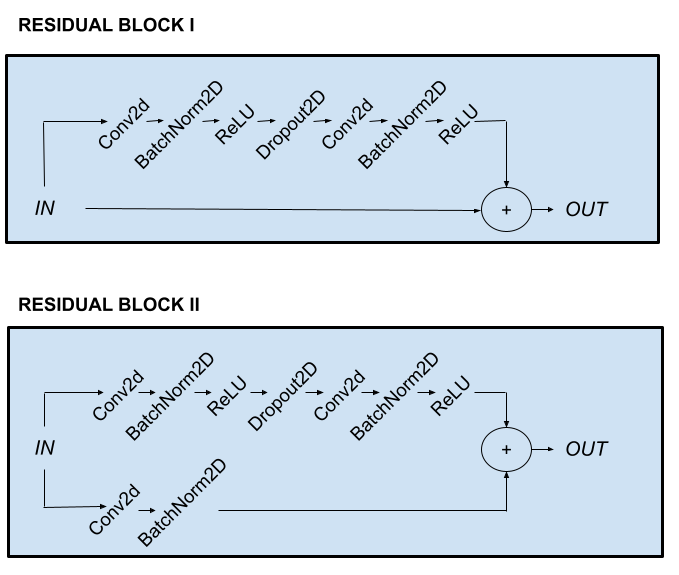
\includegraphics[width=0.8\textwidth]{figures/vi_figures/conv_block.png}
    \caption{Details of the residual network blocks from Figure~\ref{fig:starnet_arch}.
    }
    \label{fig:conv_blocks}
\end{figure}


We detail the neural network architecture. 
Figure~\ref{fig:starnet_arch} shows a schematic of the architecture, and 
Figure~\ref{fig:conv_blocks} depicts specifically 
the residual network blocks. 

The first convolutional layer (green block, Figure~\ref{fig:starnet_arch}) has 17 output-channels, a kernel size of three, a stride of one, and one pixel of padding.
All convolutional layers inside residual block 1, as well as the convolutional layers on the top row of residual block 2 (Figure~\ref{fig:conv_blocks}) also have the same parameters. 
Only the convolutional layers on the bottom row of residual block 2 are different: they still have output channels of dimension 17, 
but down-sample using a kernel size of one, and a stride of 2. 
Inside the residual blocks, the dropout layers have dropout probability of 0.11399. 

In the final fully connected block (red block, Figure~\ref{fig:starnet_arch}) have latent dimension 185, and a dropout probability of 0.013123. 

